\begin{enumerate}[label=\thesubsection.\arabic*, ref=\thesubsection.\theenumi]
    \item
    \label{question:C12-Q01}
    \label{question-short:C12-Q01} Find a vector of magnitude $\sqrt{171}$ perpendicular to both $\vec a=\myvec{1\\-2\\-3}$ and $\vec b=\myvec{3\\-1\\-2}$.

    \par
    \smallskip
    \solution

    Perpendicularity requires a vector in the null space of the matrix with rows $\vec a^T$ and $\vec b^T$:
    \begin{align*}
        M       & =\myvec{1 & -2 & -3 \\3&-1&-2}. \\
        M\vec d & =0.
    \end{align*}

    The two rows are independent, so rank--nullity gives a one-dimensional null space. Its antisymmetric cross-product basis is
    \begin{align*}
        \operatorname{Null}(M) & =\{\vec v:M\vec v=0\}.
	    \tag*{\eqref{formula:C12-Q01}}
    \end{align*}

    \par
    \begin{align*}
	    \text{Vector perpendicular to } \vec{a} \text{ and } \vec{b} \text{ is } \myvec{1 \\-7\\5}.
    \end{align*}

    Indeed,
    \begin{align*}
	    \vec a^T\myvec{1\\-7\\5} & =1+14-15=0. \\
	    \vec b^T\myvec{1\\-7\\5} & =3+7-10=0.
    \end{align*}

    Every admissible vector is therefore $\vec d=t(1,-7,5)^T$. Since
    \begin{align*}
        \|(1,-7,5)^T\|^2 & =1+49+25=75,
    \end{align*}

    the magnitude condition gives $75t^2=171$, or $t=\pm\sqrt{57}/5$. Hence
    \begin{align*}
        \vec d & =\pm\frac{\sqrt{57}}5\myvec{1 \\-7\\5}.
    \end{align*}

    \begin{figure}[H]
        \centering
        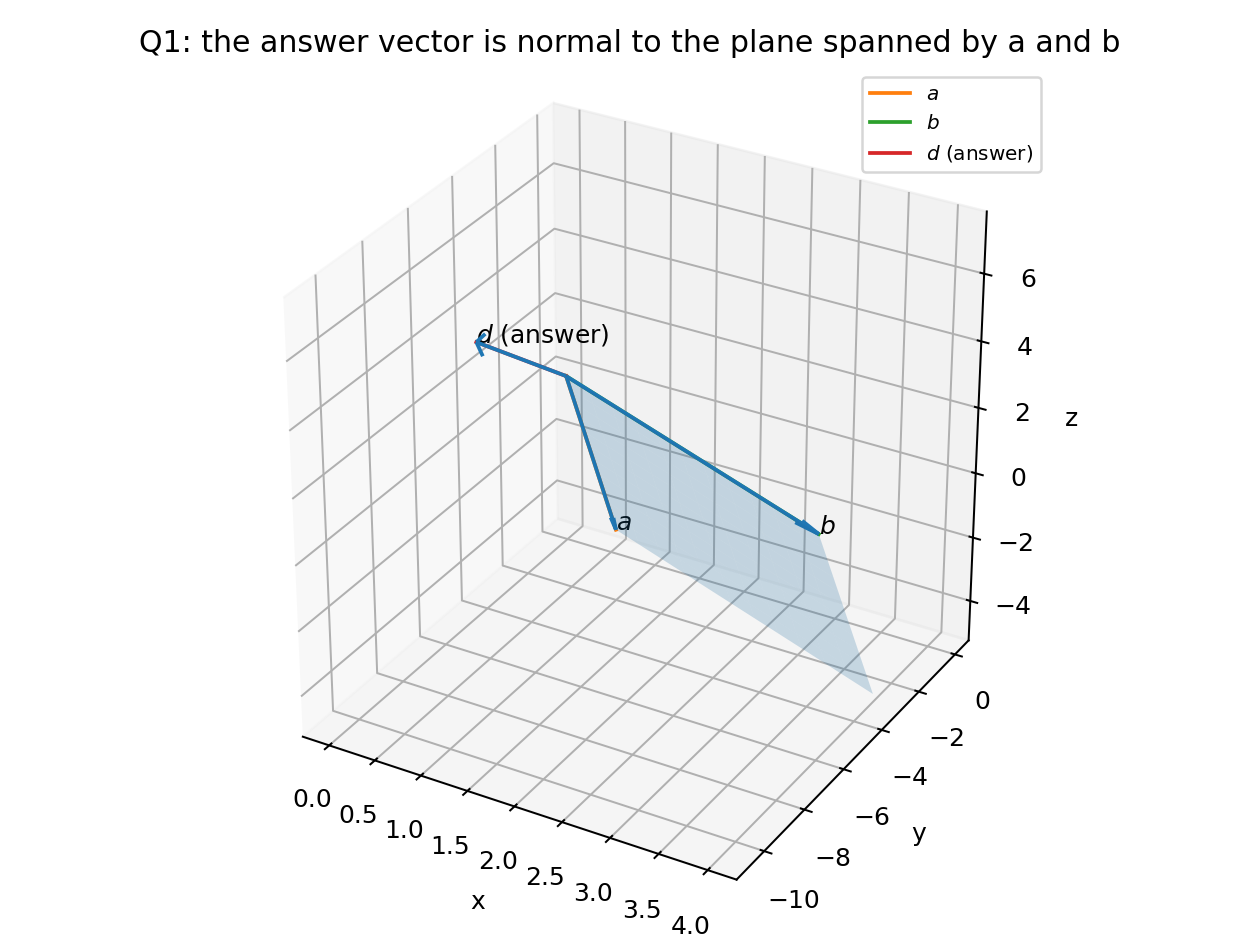
\includegraphics[width=0.96\linewidth]{12/figs/Q01.png}
    \end{figure}

    The following code verifies the solution.

    \begin{lstlisting}[frame=single, basicstyle=\rmfamily, escapeinside={(*@}{@*)}]
(*@\makebox[\dimexpr\linewidth-2\fboxsep-2\fboxrule\relax][c]{12/codes/Q01.py}@*)
    \end{lstlisting}


    \item
    \label{question:C12-Q05}
    \label{question-short:C12-Q05} Let $\vec a=\myvec{1\\4\\2}$, $\vec b=\myvec{3\\-2\\7}$ and $\vec c=\myvec{2\\-1\\4}$. Find $\vec d$ perpendicular to both $\vec a,\vec b$ with $\vec c\cdot\vec d=27$.

    \par
    \smallskip
    \solution

Perpendicularity requires a vector in the null space of the matrix with rows $\vec a^T$ and $\vec b^T$:
    \begin{align*}
        M       & =\myvec{1 & 4 & 2 \\3&-2&7}. \\
        M\vec d & =0.
    \end{align*}

    The two rows are independent, so rank--nullity gives a one-dimensional null space. Its antisymmetric cross-product basis is
    \begin{align*}
        \operatorname{Null}(M) & =\{\vec v:M\vec v=0\}.
	    \tag*{\eqref{formula:C12-Q01}}
    \end{align*}

    \par
    \begin{align*}
         \text{Vector perpendicular to } \vec{a} \text{ and } \vec{b} \text{ is } \myvec{32 \\-1\\-14}.
    \end{align*}

    Thus the complete perpendicular family is
    \begin{align*}
        \vec d & =t\myvec{32 \\-1\\-14}.
	    \tag*{\eqref{formula:C12-Q05}}
    \end{align*}

    The remaining scalar constraint selects the scale. First,
    \begin{align*}
	    \vec c^T \myvec{32\\-1\\-14} & =2(32)+(-1)(-1)+4(-14)=64+1-56=9.
    \end{align*}

    Therefore $9t=27$, so $t=3$ and
    \begin{align*}
        \vec d & =\myvec{96 \\-3\\-42}.
    \end{align*}

    The inner products $\vec a^T \vec d=0$ and $\vec b^T \vec d=0$, together with $\vec c^T \vec d=27$, verify the corrected result.

    \begin{figure}[H]
        \centering
        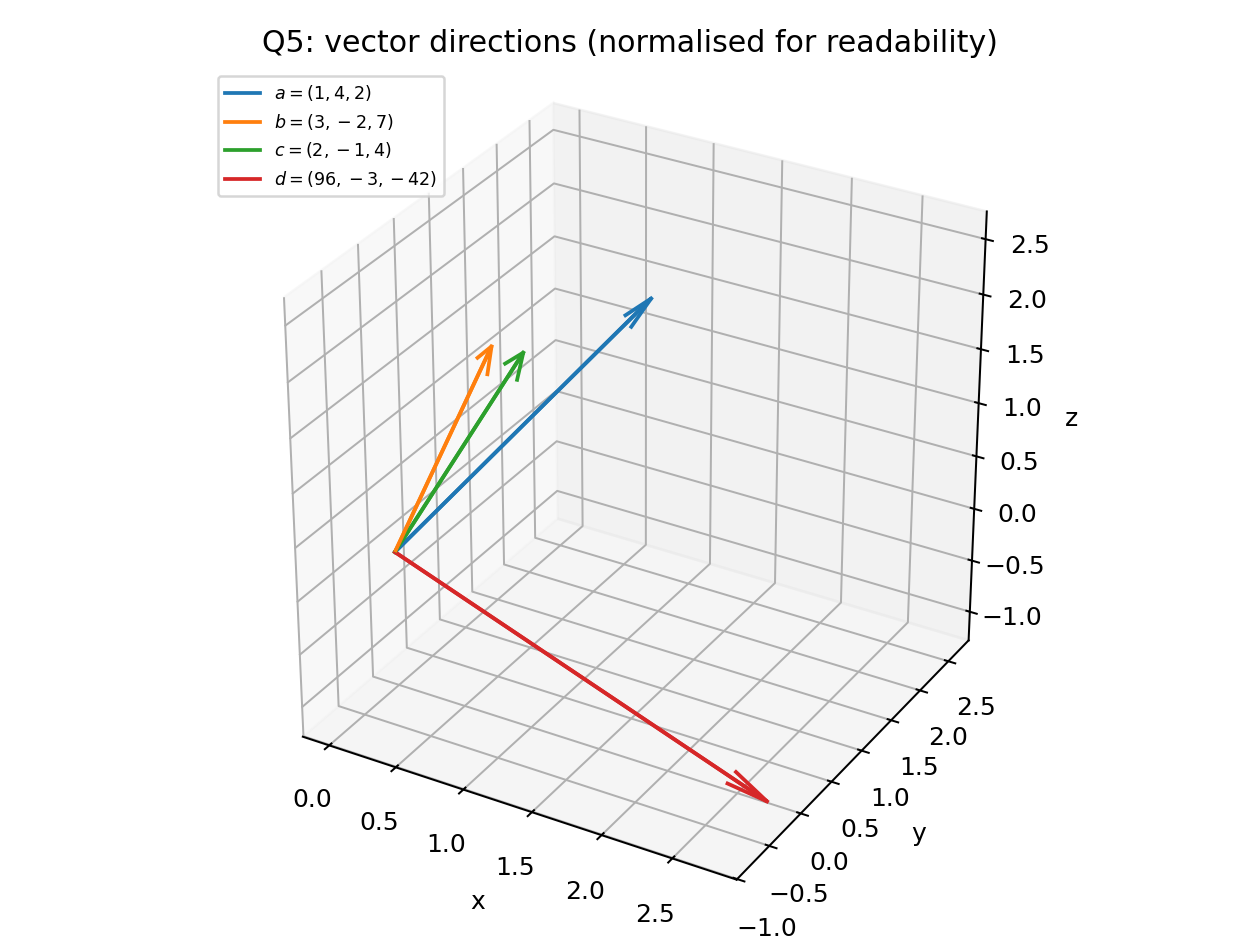
\includegraphics[width=0.96\linewidth]{12/figs/Q05.png}
    \end{figure}

    The following code verifies the solution.

    \begin{lstlisting}[frame=single, basicstyle=\rmfamily, escapeinside={(*@}{@*)}]
(*@\makebox[\dimexpr\linewidth-2\fboxsep-2\fboxrule\relax][c]{12/codes/Q05.py}@*)
    \end{lstlisting}


    \item
    \label{question:C12-Q06}
    \label{question-short:C12-Q06} Find the shortest distance between $\vec r=(1,2,3)+\lambda(2,3,4)$ and $\vec r=(2,4,5)+\mu(4,6,8)$.

    \par
    \smallskip
    \solution

    The direction vectors $(2,3,4)$ and $(4,6,8)$ are parallel. Choose one point on each line and form the joining vector
    \begin{align*}
        \vec v & =(2,3,4)^T,\qquad \vec w=(2,4,5)^T-(1,2,3)^T=(1,2,2)^T.
    \end{align*}

    Only the component of $\vec w$ orthogonal to the common direction contributes to the shortest distance. The projection-residual operator is
    \begin{align*}
        P_\perp & =I-\frac{\vec v\vec v^T}{\vec v^T\vec v}.
	    \tag*{\eqref{formula:C12-Q06}}
    \end{align*}

    \par
    \begin{align*}
        d & =\|P_\perp\vec w\|=\frac{\|\vec w\times\vec v\|}{\|\vec v\|}
	    \tag*{\eqref{formula:C12-Q06-S01}}
    \end{align*}

    \par
    Here
    \begin{align*}
        \vec w\times\vec v     & =\myvec{2   \\0\\-1}. \\
        \|\vec w\times\vec v\| & =\sqrt5.    \\
        \|\vec v\|             & =\sqrt{29}.
    \end{align*}

    Consequently,
    \begin{align*}
        d & =\sqrt{\frac5{29}}.
    \end{align*}

    The cross product is orthogonal to $\vec v$, so the residual satisfies the required projection consistency check.

    \begin{figure}[H]
        \centering
        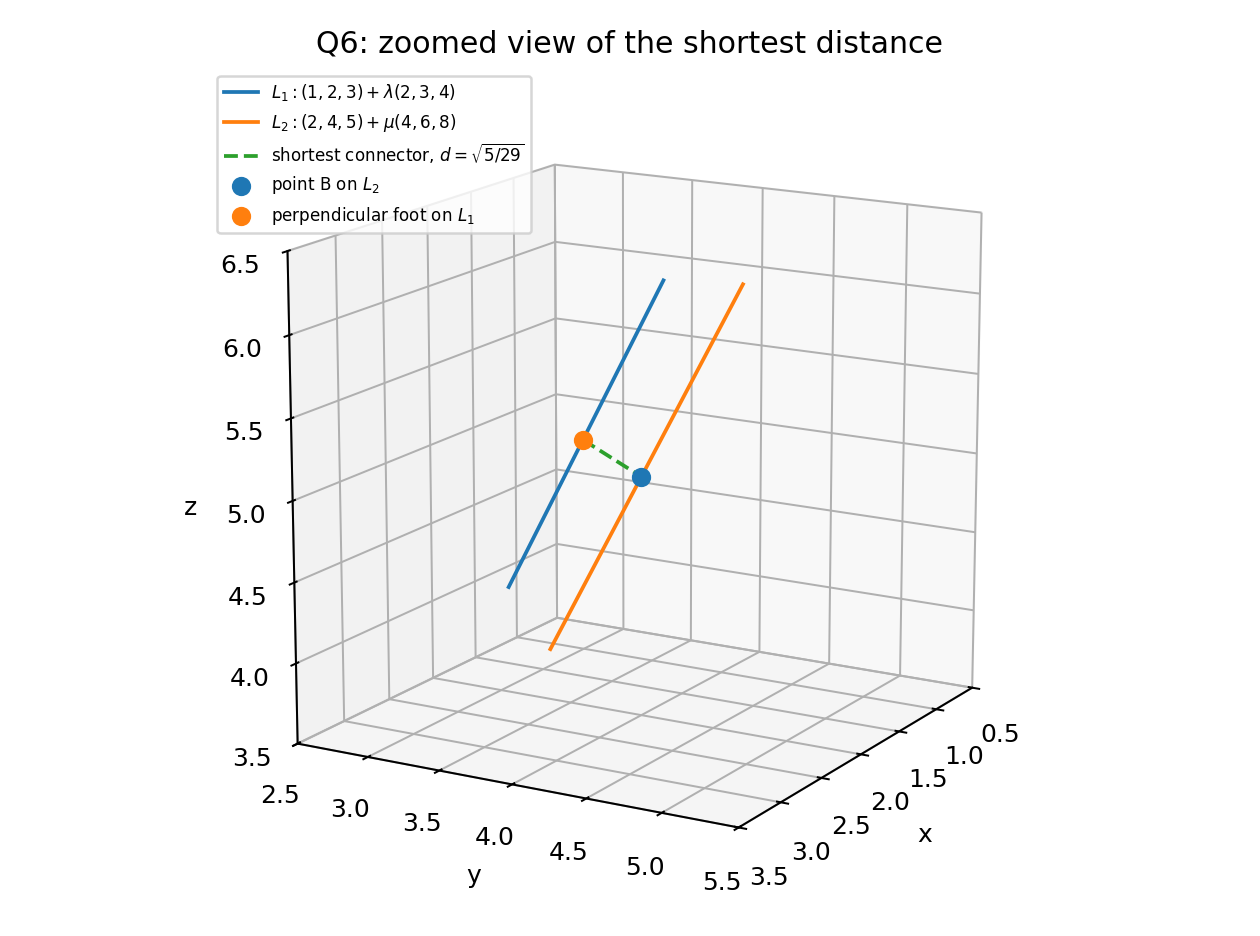
\includegraphics[width=0.96\linewidth]{12/figs/Q06.png}
    \end{figure}

    The following code verifies the solution.

    \begin{lstlisting}[frame=single, basicstyle=\rmfamily, escapeinside={(*@}{@*)}]
(*@\makebox[\dimexpr\linewidth-2\fboxsep-2\fboxrule\relax][c]{12/codes/Q06.py}@*)
    \end{lstlisting}


    \par
    \medskip
    \par
    \smallskip

    \item
    \label{question:C12-Q10}
    \label{question-short:C12-Q10} Find the plane through the intersection of $2x+y-z=3$ and $5x-3y+4z+9=0$ that is parallel to $\frac{x-1}{2}=\frac{y-3}{-4}=\frac{5-z}{-5}$.

    \par
    \smallskip
    \solution

    Let
    \begin{align*}
        P_1 & =2x+y-z-3.   \\
        P_2 & =5x-3y+4z+9.
    \end{align*}

    Every plane through the intersection line belongs to the affine pencil $P_1+\lambda P_2=0$. Its normal is
    \begin{align*}
	    \vec n(\lambda) & = \myvec{2+5\lambda\\1-3\lambda\\-1+4\lambda}.
    \end{align*}

    The direction of the given line is $\vec d=(2,-4,5)^T$. The required parallelism condition is
    \begin{align*}
        (\vec n_1+\lambda\vec n_2)^T\vec d & =0.
	    \tag*{\eqref{formula:C12-Q10}}
    \end{align*}

    \par
    Substitution gives
    \begin{align*}
        2(2+5\lambda)-4(1-3\lambda)+5(-1+4\lambda) & =0,
    \end{align*}

    so $-5+42\lambda=0$ and $\lambda=5/42$. Multiplying the pencil by 42 yields
    \begin{align*}
        42P_1+5P_2 & =0
        \Longrightarrow 109x+27y-22z-81=0.
    \end{align*}

    The plane contains the intersection line by construction, and its normal has zero inner product with the given line direction.

    \begin{figure}[H]
        \centering
        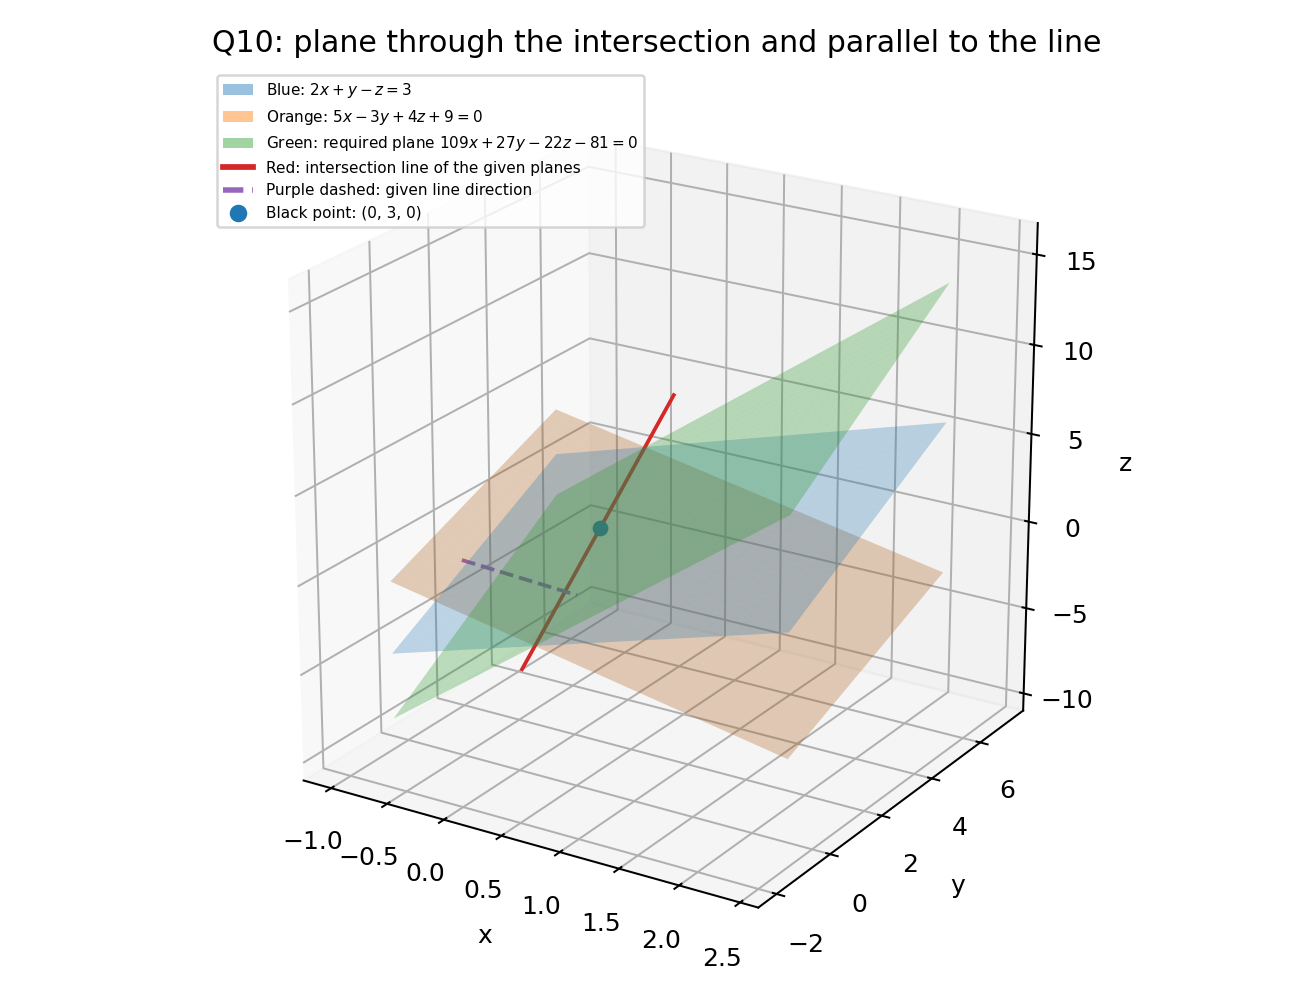
\includegraphics[width=0.96\linewidth]{12/figs/Q10.png}
    \end{figure}

    The following code verifies the solution.

    \begin{lstlisting}[frame=single, basicstyle=\rmfamily, escapeinside={(*@}{@*)}]
(*@\makebox[\dimexpr\linewidth-2\fboxsep-2\fboxrule\relax][c]{12/codes/Q10.py}@*)
    \end{lstlisting}


    \item
    \label{question:C12-Q15}
    \label{question-short:C12-Q15} Find where the line through $\vec{A}(3,4,1)$ and $\vec B(5,1,6)$ meets the plane through $\vec P(2,1,2)$, $\vec Q(3,1,0)$ and $\vec R(4,-2,1)$.

    \par
    \smallskip
    \solution

    The two plane-edge vectors are
    \begin{align*}
	    \vec{Q-P} & =(1,0,-2)^T.  \\
	    \vec{R-P} & =(2,-3,-1)^T.
    \end{align*}

    Their cross product is proportional to $(2,1,1)^T$, so the plane equation is
    \begin{align*}
        2(x-2)+(y-1)+(z-2) & =0
        \Longrightarrow 2x+y+z=7.
    \end{align*}

    The line direction is $B-A=(2,-3,5)^T$. Its affine representation is
    \begin{align*}
        \vec r & =\vec A+t\vec d.
	    \tag*{\eqref{formula:C12-Q15}}
    \end{align*}

    \par
    Thus
    \begin{align*}
        \vec r & =(3,4,1)^T+t(2,-3,5)^T.
    \end{align*}

    Substitution into the plane gives
    \begin{align*}
        2(3+2t)+(4-3t)+(1+5t) & =7
        \Longrightarrow 11+6t=7
        \Longrightarrow t=-\frac23.
    \end{align*}

    The intersection point is therefore
    \begin{align*}
        & \left(\frac53,6,-\frac73\right)^T.
    \end{align*}

    Putting this point back into $2x+y+z$ gives $10/3+6-7/3=7$, which verifies the incidence condition.

    \begin{figure}[H]
        \centering
        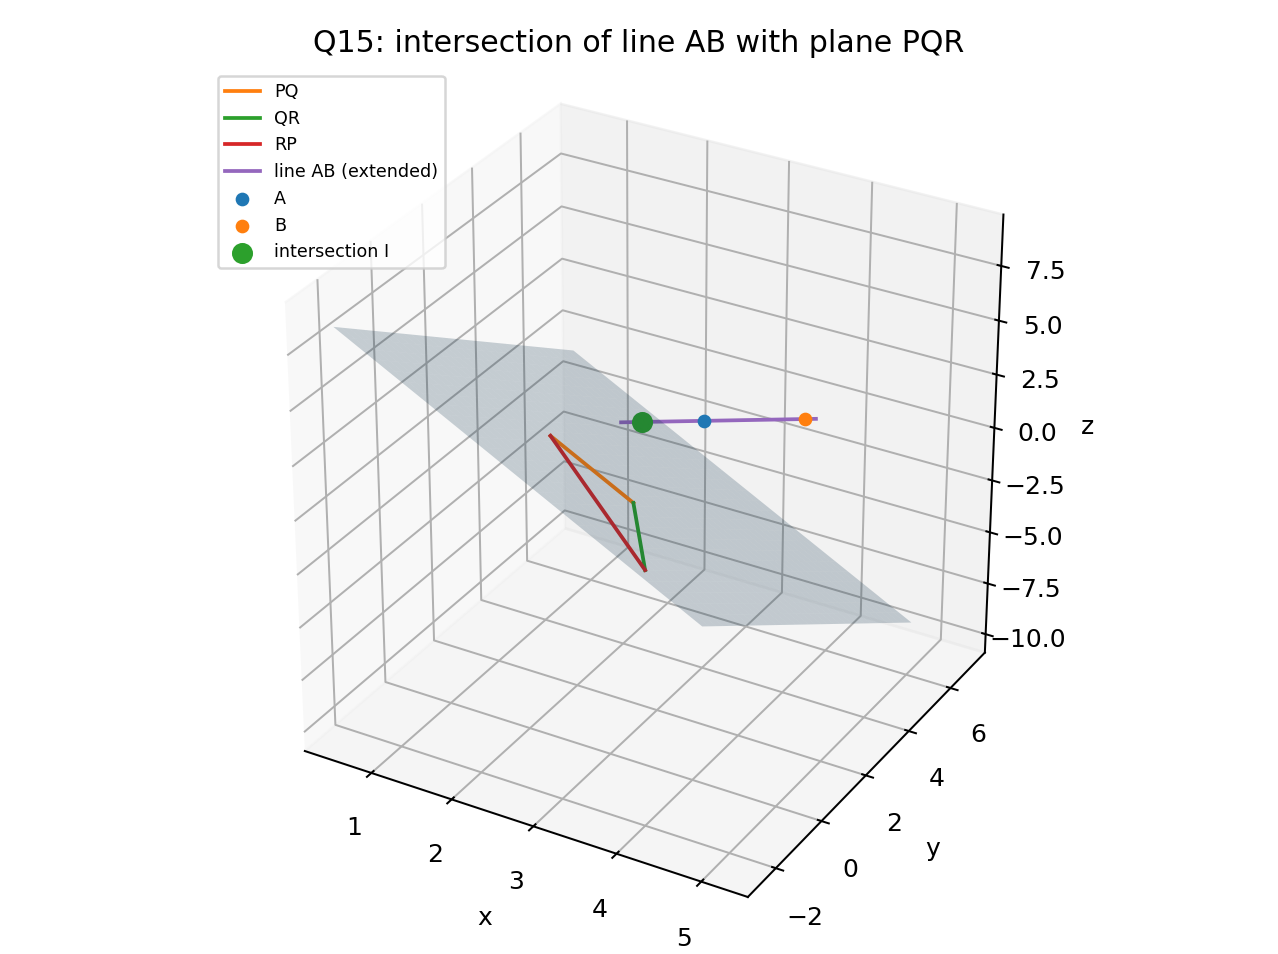
\includegraphics[width=0.96\linewidth]{12/figs/Q15.png}
    \end{figure}

    The following code verifies the solution.
\\
    \begin{lstlisting}[frame=single, basicstyle=\rmfamily, escapeinside={(*@}{@*)}]
(*@\makebox[\dimexpr\linewidth-2\fboxsep-2\fboxrule\relax][c]{12/codes/Q15.py}@*)
    \end{lstlisting}



    \item
    \label{question:C12-Q28}
    \label{question-short:C12-Q28} If $A=\myvec{\cos\theta&\sin\theta\\\sin\theta&\cos\theta}$, find $\det(A^n)$ for natural $n$.

    \par
    \smallskip
    \solution

    The symmetric matrix has eigenvectors $\vec q_1=(1,1)^T$ and $\vec q_2=(1,-1)^T$. Their eigenvalues are
    \begin{align*}
        \lambda_1 & =\cos\theta+\sin\theta. \\
        \lambda_2 & =\cos\theta-\sin\theta.
    \end{align*}

    $\det A=\lambda_1\lambda_2$ and raises each eigenvalue to the $n$th power. Using the determinant-power identity,
    \begin{align*}
        \det(A^n) & =(\det A)^n.
	    \tag*{\eqref{formula:C12-Q28}}
    \end{align*}

    \par
    We obtain
    \begin{align*}
        \det(A^n) & =(\lambda_1\lambda_2)^n
        =\bigl((\cos\theta+\sin\theta)(\cos\theta-\sin\theta)\bigr)^n
        =(\cos2\theta)^n.
    \end{align*}


    \item
    \label{question:C12-Q30}
    \label{question-short:C12-Q30} Find the inverse of $\myvec{0&1&2\\1&2&3\\3&1&0}$ using elementary row operations.

    \par
    \smallskip
    \solution

\[
A=\myvec{
0&1&2\\
1&2&3\\
3&1&0
}
\]

\[
\myvec{
0&1&2&\big|&1&0&0\\
1&2&3&\big|&0&1&0\\
3&1&0&\big|&0&0&1
}
\]

\[
R_1\leftrightarrow R_2
\]

\[
\myvec{
1&2&3&\big|&0&1&0\\
0&1&2&\big|&1&0&0\\
3&1&0&\big|&0&0&1
}
\]

\[
R_3\rightarrow R_3-3R_1
\]

\[
\myvec{
1&2&3&\big|&0&1&0\\
0&1&2&\big|&1&0&0\\
0&-5&-9&\big|&0&-3&1
}
\]

\[
R_3\rightarrow R_3+5R_2
\]

\[
\myvec{
1&2&3&\big|&0&1&0\\
0&1&2&\big|&1&0&0\\
0&0&1&\big|&5&-3&1
}
\]

\[
R_2\rightarrow R_2-2R_3
\]

\[
\myvec{
1&2&3&\big|&0&1&0\\
0&1&0&\big|&-9&6&-2\\
0&0&1&\big|&5&-3&1
}
\]

\[
R_1\rightarrow R_1-3R_3
\]

\[
\myvec{
1&2&0&\big|&-15&10&-3\\
0&1&0&\big|&-9&6&-2\\
0&0&1&\big|&5&-3&1
}
\]

\[
R_1\rightarrow R_1-2R_2
\]

\[
\myvec{
1&0&0&\big|&3&-2&1\\
0&1&0&\big|&-9&6&-2\\
0&0&1&\big|&5&-3&1
}
\]

\[
A^{-1}=
\myvec{
3&-2&1\\
-9&6&-2\\
5&-3&1
}
\]

\[
\begin{aligned}
AA^{-1}
&=
\myvec{
0&1&2\\
1&2&3\\
3&1&0
}
\myvec{
3&-2&1\\
-9&6&-2\\
5&-3&1
}\\[6pt]
&=
\myvec{
1&0&0\\
0&1&0\\
0&0&1
}\\
&=I
\end{aligned}
\]


    The following code verifies the solution.

    \begin{lstlisting}[frame=single, basicstyle=\rmfamily, escapeinside={(*@}{@*)}]
(*@\makebox[\dimexpr\linewidth-2\fboxsep-2\fboxrule\relax][c]{12/codes/Q30.py}@*)
    \end{lstlisting}



    \item
    \label{question:C12-Q48}
    \label{question-short:C12-Q48} Discuss continuity and differentiability of $f(x)=|x|+|x-1|$ on $(-1,2)$.

    \par
    \smallskip
    \solution

    The absolute-value characteristic changes branch at $x=0$ and $x=1$. Resolving the signs gives
    \begin{align*}
        f(x) & =|x|+|x-1|=
        \begin{cases}1-2x,&-1<x<0,\\1,&0\le x<1,\\2x-1,&1\le x<2.
        \end{cases}
    \end{align*}

    At the first breakpoint,
    \begin{align*}
        \lim_{x\to0^-}f(x) & =1=f(0)=\lim_{x\to0^+}f(x),
    \end{align*}

    and at the second,
    \begin{align*}
        \lim_{x\to1^-}f(x) & =1=f(1)=\lim_{x\to1^+}f(x).
    \end{align*}

    Thus the function is continuous throughout $(-1,2)$. Its one-sided derivatives are
    \begin{align*}
        f'_-(0) & =-2. \\
        f'_+(0) & =0.  \\
        f'_-(1) & =0.  \\
        f'_+(1) & =2.
    \end{align*}

    The slopes disagree at both breakpoints, so f is not differentiable at 0 or 1, but
is differentiable elsewhere.


	\begin{figure}[H]
        \centering
        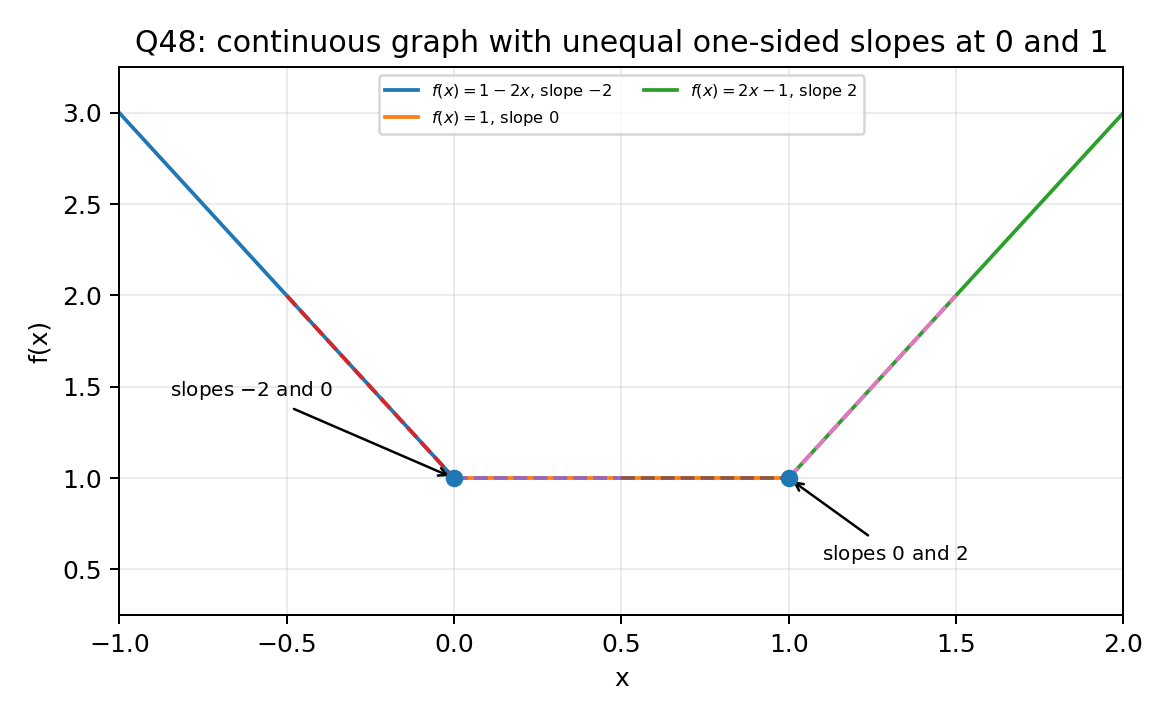
\includegraphics[width=0.92\linewidth]{12/figs/Q48.png}
    \end{figure}

    The following code verifies the solution.

    \begin{lstlisting}[frame=single, basicstyle=\rmfamily, escapeinside={(*@}{@*)}]
(*@\makebox[\dimexpr\linewidth-2\fboxsep-2\fboxrule\relax][c]{12/codes/Q48.py}@*)
    \end{lstlisting}



    \item
    \label{question:C12-Q52}
    \label{question-short:C12-Q52} Find any point of discontinuity of $f(x)=x-|x-x^2|$, $x\in[-1,1]$.

    \par
    \smallskip
    \solution

    Factor the expression inside the absolute value:
    \begin{align*}
        x-x^2 & =x(1-x).
	    \tag*{\eqref{formula:C12-Q52}}
    \end{align*}

    \par
    On $[-1,1]$, this quantity is nonnegative for $0\le x\le1$ and nonpositive for $-1\le x\le0$. The piecewise nonlinear map is therefore
    \begin{align*}
        f(x) & =
        \begin{cases}2x-x^2,&-1\le x\le0,\\x^2,&0\le x\le1.
        \end{cases}
    \end{align*}

    At the switching point, both branches give $f(0)=0$. Moreover,
    \begin{align*}
        \lim_{x\to0^-}(2x-x^2) & =0=f(0)=\lim_{x\to0^+}x^2.
    \end{align*}

    Thus there is no discontinuity on the domain.


    \begin{figure}[H]
        \centering
        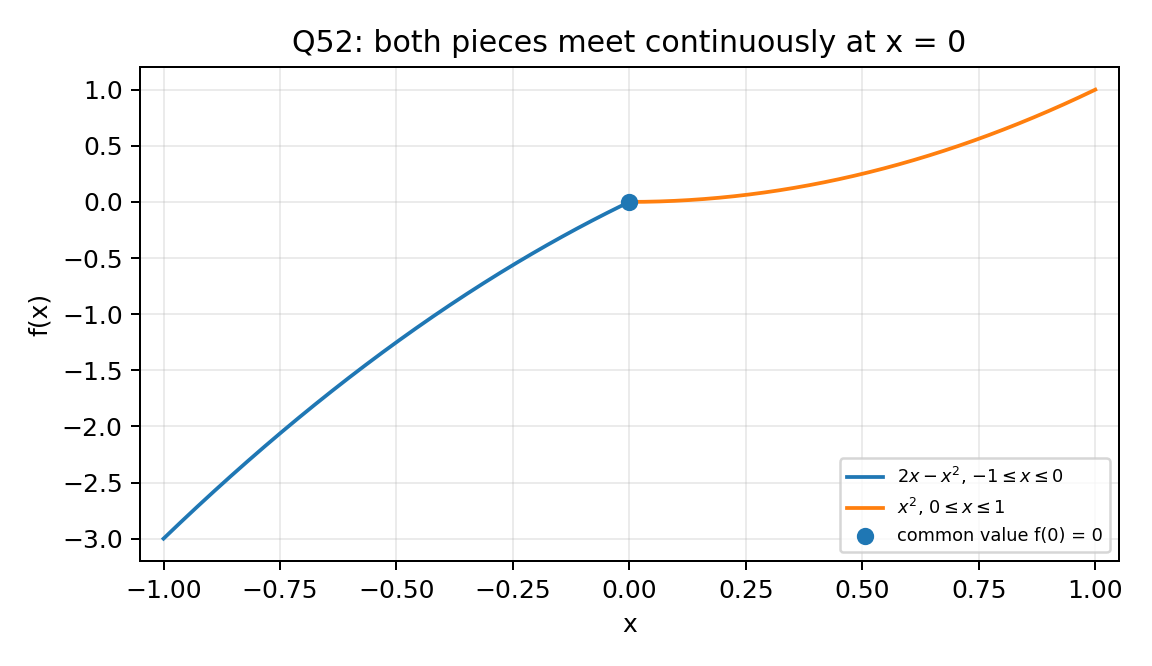
\includegraphics[width=0.92\linewidth]{12/figs/Q52.png}
    \end{figure}

    The following code verifies the solution.

    \begin{lstlisting}[frame=single, basicstyle=\rmfamily, escapeinside={(*@}{@*)}]
(*@\makebox[\dimexpr\linewidth-2\fboxsep-2\fboxrule\relax][c]{12/codes/Q52.py}@*)
    \end{lstlisting}


    \item
    \label{question:C12-Q53}
    \label{question-short:C12-Q53} A man steps forward with probability $0.4$ and backward with probability $0.6$. Find the probability that after 5 steps he is one step away from his starting point.

    \par
    \smallskip
    \solution


    After five steps, displacement $+1$ requires three forward and two backward steps, while displacement $-1$ requires two forward and three backward steps. Let X denote the net displacement.
    \begin{align*}
        P(|X|=1) & =\binom53(0.4)^3(0.6)^2+\binom52(0.4)^2(0.6)^3.
	    \tag*{\eqref{formula:C12-Q53}}
    \end{align*}

    Numerically,
    \begin{align*}
        \binom53(0.064)(0.36)+\binom52(0.16)(0.216) & =0.3456+0.2304=0.576.
    \end{align*}

    The two cases are disjoint and exhaust the requested one-step displacement events.

\begin{table}[H]
    \centering
    \begin{tabular}{|c|c|c|c|c|c|c|}
        \hline
        $x$ & $-5$ & $-3$ & $-1$ & $1$ & $3$ & $5$ \\ \hline
        $P(X=x)$ & $\frac{1}{32}$ & $\frac{5}{32}$ & $\frac{10}{32}$ & $\frac{10}{32}$ & $\frac{5}{32}$ & $\frac{1}{32}$ \\ \hline
    \end{tabular}
    \caption{Probability Mass Function of the Random Walk}
    \label{tab:random-walk-pmf}
\end{table}
    \begin{figure}[H]
        \centering
        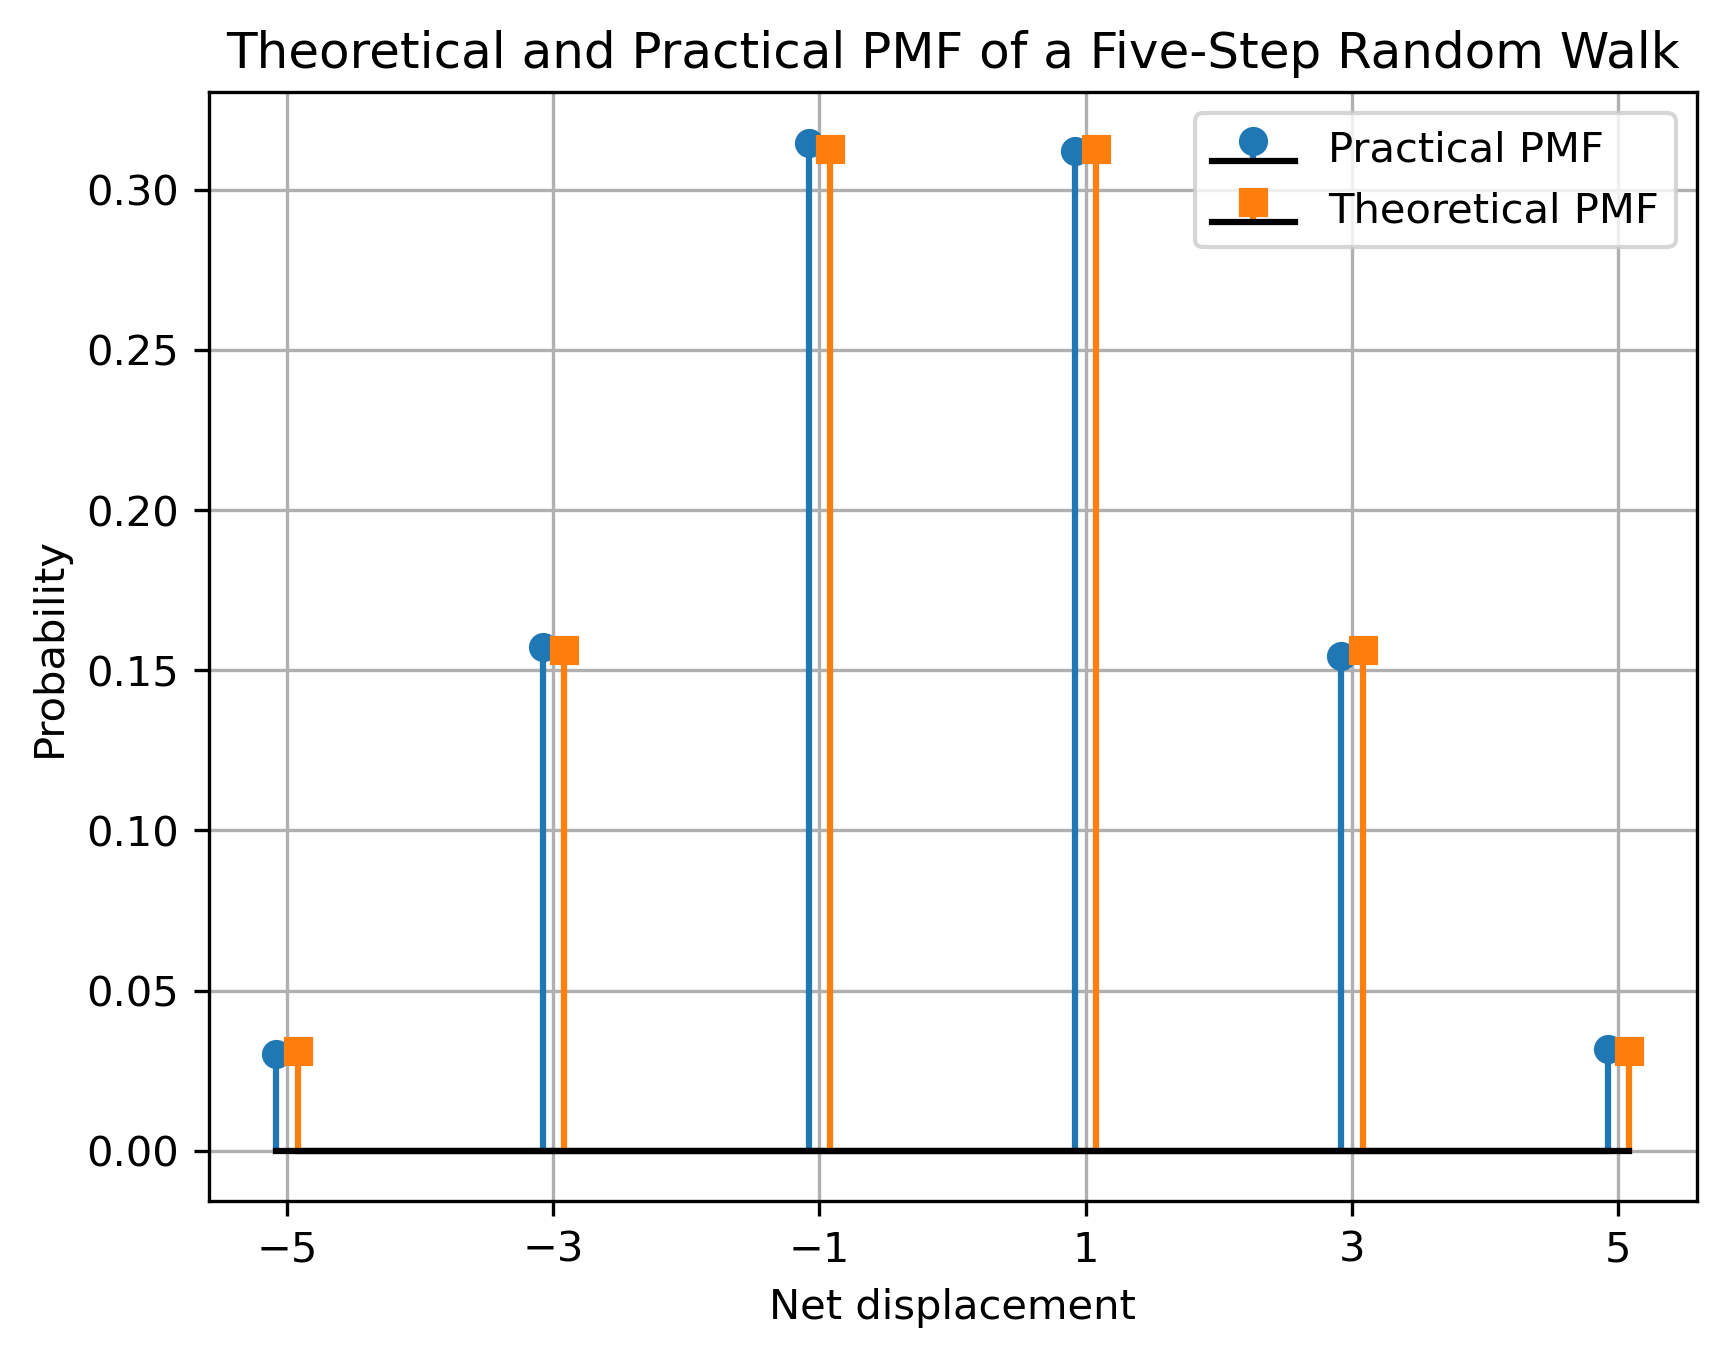
\includegraphics[width=0.92\linewidth]{12/figs/Q53.png}
    \end{figure}

    The following code generates 10,000 iterations.

\begin{lstlisting}[frame=single, basicstyle=\rmfamily, escapeinside={(*@}{@*)}]
(*@\makebox[\dimexpr\linewidth-2\fboxsep-2\fboxrule\relax][c]{12/codes/Q53/random\_walk.c}@*)
    \end{lstlisting}

    The following code verifies the solution.

    \begin{lstlisting}[frame=single, basicstyle=\rmfamily, escapeinside={(*@}{@*)}]
(*@\makebox[\dimexpr\linewidth-2\fboxsep-2\fboxrule\relax][c]{12/codes/Q53/Q53.py}@*)
    \end{lstlisting}


    \item
    \label{question:C12-Q54}
    \label{question-short:C12-Q54} A girl throws a die. If it shows 1 or 2, she tosses a coin three times; otherwise she tosses it once. Given that exactly one tail was obtained, find the probability that the die showed 3, 4, 5 or 6.

    \par
    \smallskip
    \solution

    Let $H_1$ denote die outcomes $1$ or $2$, $H_2$ denote outcomes $3,4,5,6$, and let $E$ be the event of exactly one tail. Then
    \begin{align*}
        P(H_1) & =\frac13. \\
        P(H_2) & =\frac23.
    \end{align*}

    Under $H_1$, exactly one tail in three tosses has likelihood $3(1/2)^3=3/8$; under $H_2$, exactly one tail in one toss has likelihood $1/2$. Bayes' rule is
    \begin{align*}
        P(H_2\mid E) & =\frac{P(E\mid H_2)P(H_2)}{P(E)}.
	    \tag*{\eqref{formula:C12-Q54}}
    \end{align*}

    \par
    The evidence probability is
    \begin{align*}
        P(E) & =\frac38\cdot\frac13+\frac12\cdot\frac23=\frac18+\frac13=\frac{11}{24}.
    \end{align*}

    Therefore
    \begin{align*}
        P(H_2\mid E) & =\frac{(1/2)(2/3)}{11/24}=\frac{1/3}{11/24}=\frac8{11}.
    \end{align*}

        \begin{figure}[H]
        \centering
        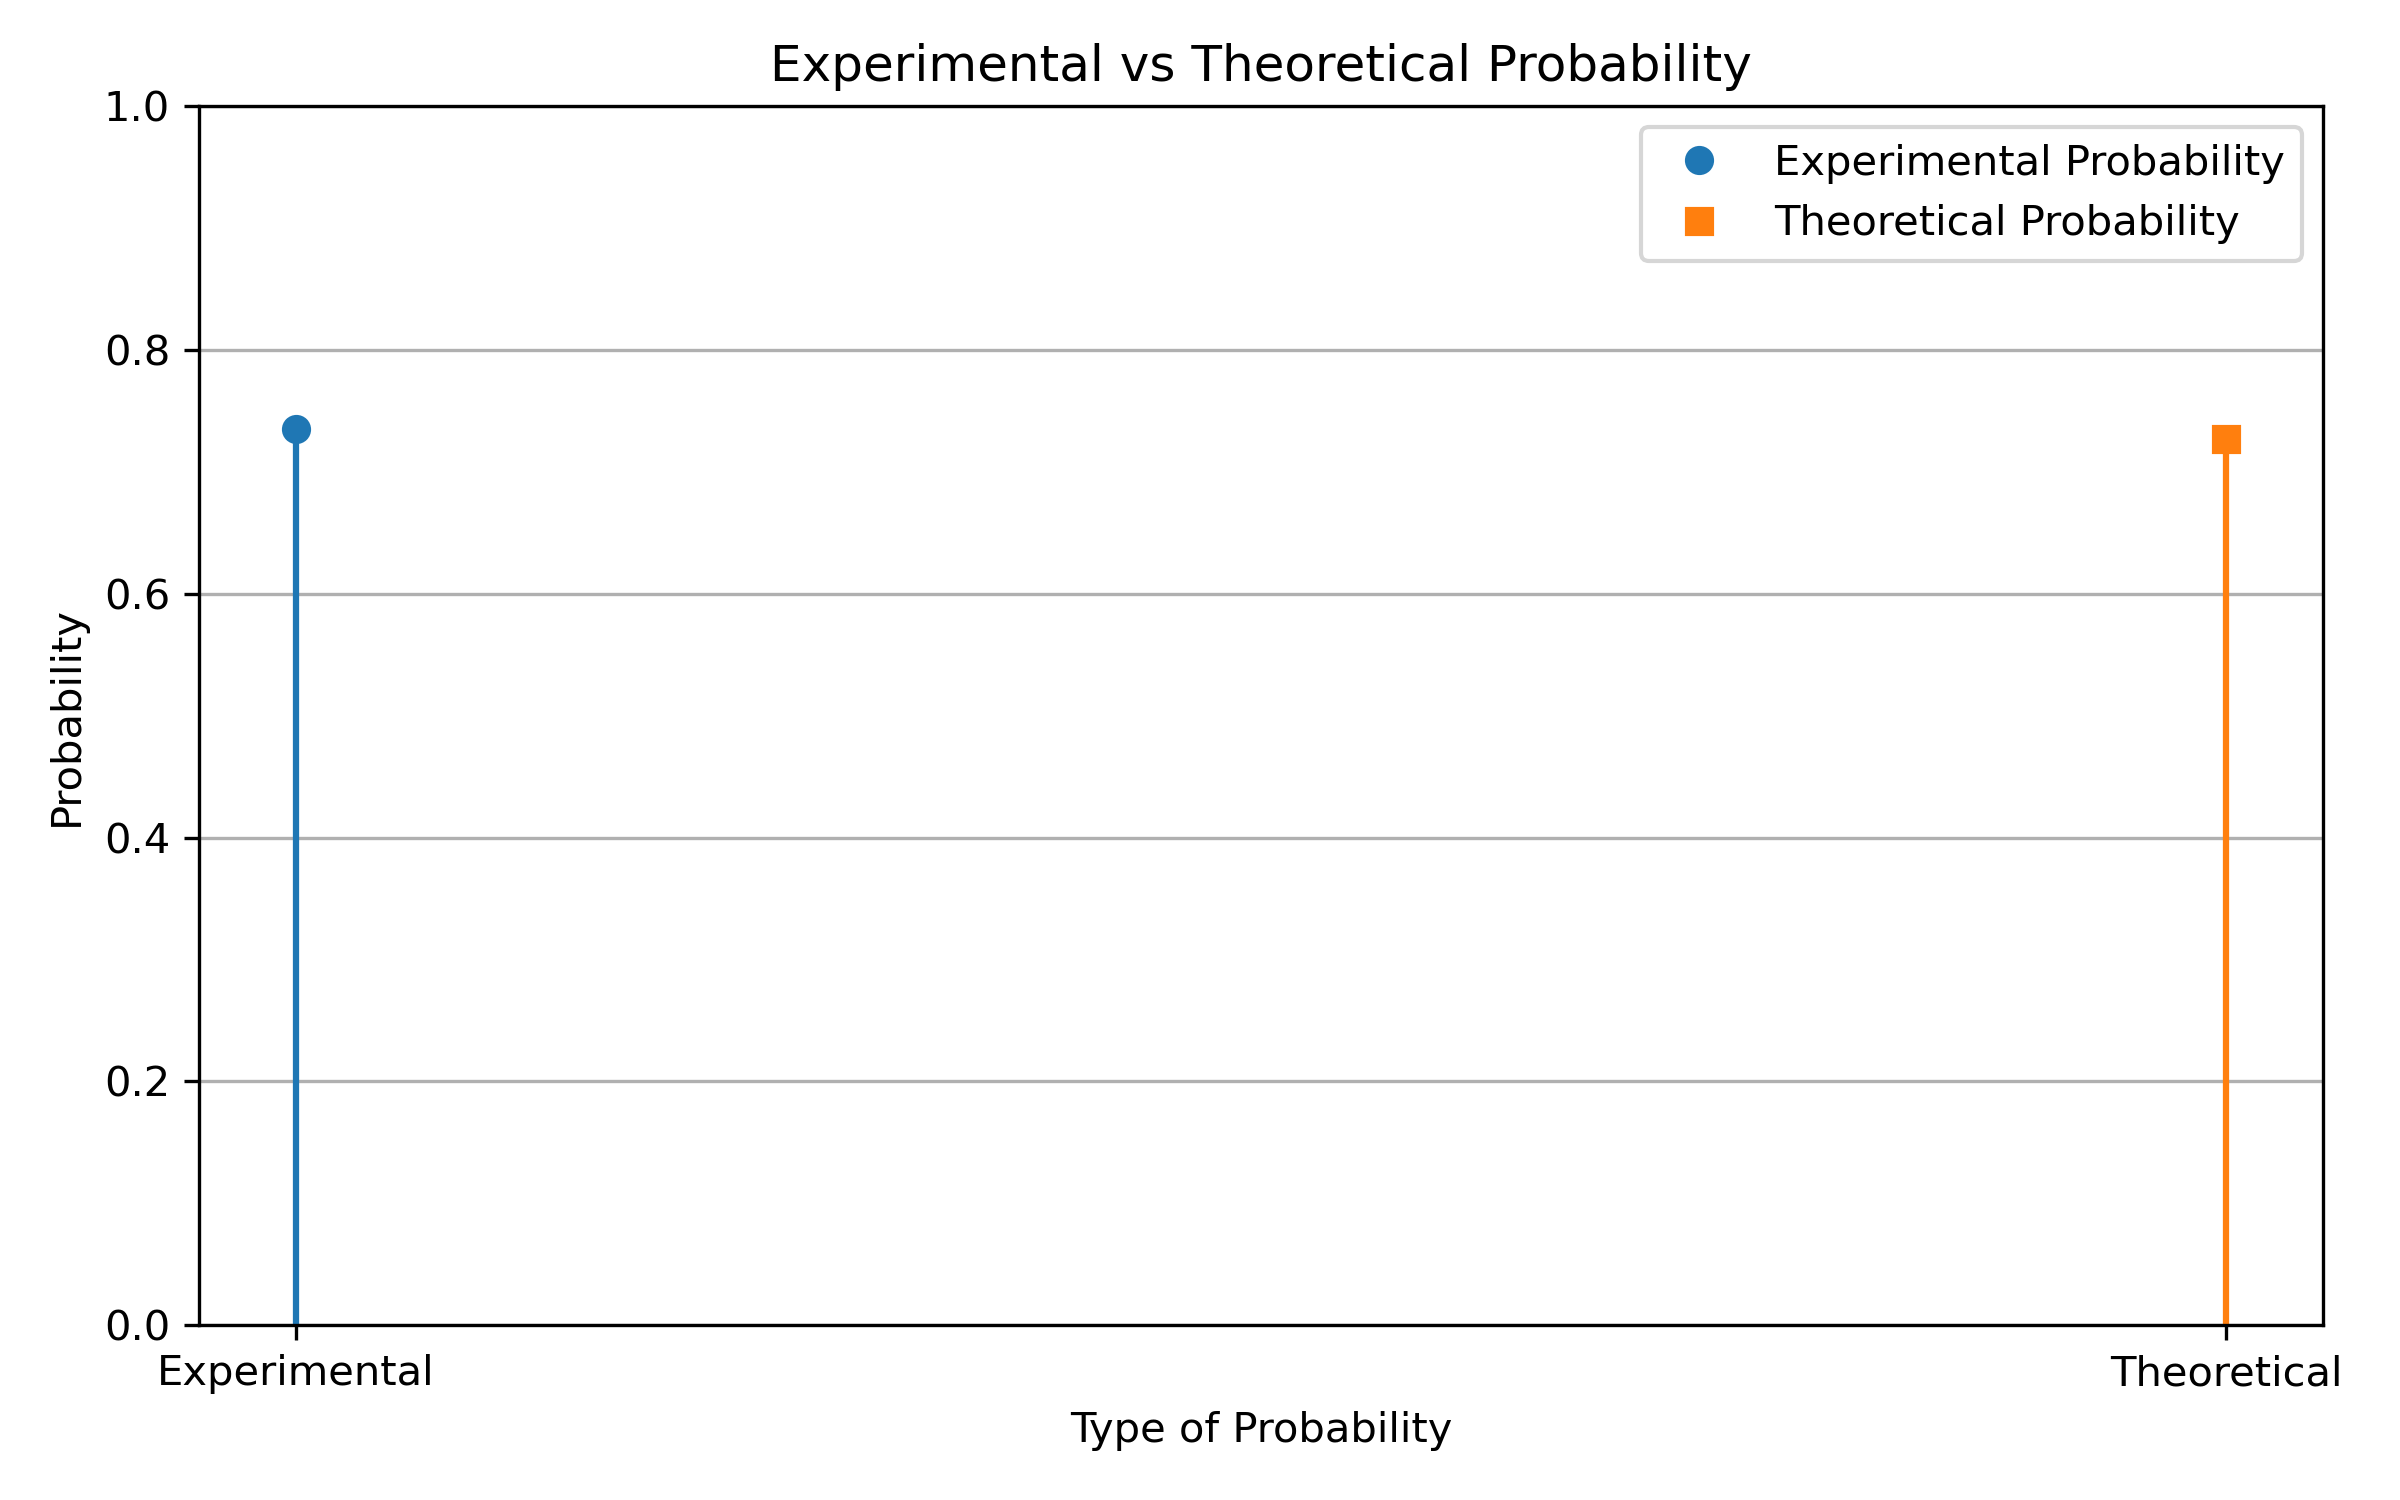
\includegraphics[width=0.92\linewidth]{12/figs/Q54.png}
    \end{figure}

    The following code generates 10,000 outcomes.
        \begin{lstlisting}[frame=single, basicstyle=\rmfamily, escapeinside={(*@}{@*)}]
(*@\makebox[\dimexpr\linewidth-2\fboxsep-2\fboxrule\relax][c]{12/codes/Q54/Q54.c}@*)
    \end{lstlisting}

    The following code verifies the solution.
        \begin{lstlisting}[frame=single, basicstyle=\rmfamily, escapeinside={(*@}{@*)}]
(*@\makebox[\dimexpr\linewidth-2\fboxsep-2\fboxrule\relax][c]{12/codes/Q54/Q54.py}@*)
    \end{lstlisting}


    \item
    \label{question:C12-Q56}
    \label{question-short:C12-Q56} In 3 trials of a binomial distribution, the probability of exactly 2 successes is 9 times the probability of 3 successes. Find the success probability.

    \par
    \smallskip
    \solution

    For three independent trials with success probability $p$,
\begin{align*}
    P(X=x) &= \binom{3}{x}p^x(1-p)^{3-x}.
    \tag*{\eqref{formula:C12-Q56}}\\
    P(X=2) &= \binom{3}{2}p^2(1-p)^{3-2} \\
           &= 3p^2(1-p). \\
    P(X=3) &= \binom{3}{3}p^3(1-p)^0 \\
           &= p^3.
\end{align*}

    The given relation produces
    \begin{align*}
        3p^2(1-p) & =9p^3
        \Longrightarrow 3p^2(1-4p)=0.
    \end{align*}

    Both roots are admissible probabilities in $[0,1]$:
    \begin{align*}
        p & =0\quad\text{or}\quad p=\frac14.
    \end{align*}

    The $p=0$ case makes both probabilities zero, so it is retained as an edge case rather than divided away.

    The following code verifies the solution.

    \begin{lstlisting}[frame=single, basicstyle=\rmfamily, escapeinside={(*@}{@*)}]
(*@\makebox[\dimexpr\linewidth-2\fboxsep-2\fboxrule\relax][c]{12/codes/Q56.py}@*)
    \end{lstlisting}


    \item
    \label{question:C12-Q57}
    \label{question-short:C12-Q57} An urn contains 3 red and 5 black balls. A ball is drawn, its colour recorded and returned, and 2 more balls of that colour are added. Then two balls are drawn without replacement. Find the probability both are red.

    \par
    \smallskip
    \solution

    Condition on the colour of the reinforced first draw. The initial state is $(R,B)=(3,5)$, so the branch probabilities are $3/8$ and $5/8$. After a red first draw the state is $(5,5)$; after a black first draw it is $(3,7)$. The law of total probability is
    \begin{align*}
        P(E) & =\sum_iP(E\mid S_i)P(S_i).
	    \tag*{\eqref{formula:C12-Q57}}
    \end{align*}

    \par
    For the red branch,
    \begin{align*}
        P(RR\mid R_1) & =\frac5{10}\frac4{9}=\frac29.
    \end{align*}

    For the black branch,
    \begin{align*}
        P(RR\mid B_1) & =\frac3{10}\frac2{9}=\frac1{15}.
    \end{align*}

    Combining the mutually exclusive branches,
    \begin{align*}
        P(RR) & =\frac38\frac29+\frac58\frac1{15}
        =\frac1{12}+\frac1{24}=\frac18.
    \end{align*}

    The state update is applied before the two final draws, preserving the reinforcement dependence.

    The following code verifies the solution.

    \begin{lstlisting}[frame=single, basicstyle=\rmfamily, escapeinside={(*@}{@*)}]
(*@\makebox[\dimexpr\linewidth-2\fboxsep-2\fboxrule\relax][c]{12/codes/Q57.py}@*)
    \end{lstlisting}


    \par
    \medskip
    \par
    \smallskip

    \item
    \label{question:C12-Q59}
    \label{question-short:C12-Q59} Solve graphically: minimise $z=3x+5y$ subject to $x+2y\ge10$, $x+y\ge6$, $3x+y\ge8$, $x,y\ge0$.

    \par
    \smallskip
    \solution



Let
\[
\vec{x}=\myvec{x\\y}
\quad\text{and}\quad
\vec{c}=\myvec{3\\5}.
\]
Write the constraints as
\[
A\vec{x}\geq\vec{b},
\qquad
\vec{x}\geq\vec{0},
\]
where
\[
A=\myvec{1&2\\1&1\\3&1},
\qquad
\vec{b}=\myvec{10\\6\\8}.
\]

The objective function is
\[
Z=\vec{c}^{\,T}\vec{x}.
\]

\par
\medskip
\noindent
\par
\smallskip

The boundary lines are
\[
\begin{aligned}
x+2y&=10,\\
x+y&=6,\\
3x+y&=8.
\end{aligned}
\]

The intersection of the first and second lines is
\[
\begin{aligned}
x+2y&=10,\\
x+y&=6.
\end{aligned}
\]
Subtracting the second equation from the first,
\[
y=4,\qquad x=2.
\]
Thus, one feasible vertex is
\[
\vec{x}_1=\myvec{2\\4}.
\]

The intersection of the second and third lines is
\[
\begin{aligned}
x+y&=6,\\
3x+y&=8.
\end{aligned}
\]
Subtracting the first equation from the second,
\[
2x=2\implies x=1.
\]
Therefore,
\[
y=5.
\]
Thus, another feasible vertex is
\[
\vec{x}_2=\myvec{1\\5}.
\]

Putting $x=0$ in the constraints gives
\[
y\geq 5,\qquad y\geq 6,\qquad y\geq 8.
\]
Hence, the corresponding feasible vertex is
\[
\vec{x}_3=\myvec{0\\8}.
\]

Similarly, putting $y=0$ in the constraints gives
\[
x\geq 10,\qquad x\geq 6,\qquad 3x\geq 8.
\]
Hence, the corresponding feasible vertex is
\[
\vec{x}_4=\myvec{10\\0}.
\]

Therefore, the feasible vertices are the following $2\times 1$
point matrices:
\[
\myvec{0\\8},
\quad
\myvec{1\\5},
\quad
\myvec{2\\4},
\quad
\myvec{10\\0}.
\]

\par
\medskip
\noindent
\par
\smallskip

The linear programming vertex rule requires evaluating $Z$
at each feasible vertex:
\[
Z=3x+5y.
\]

\[
\begin{array}{c|cccc}
\vec{x}
&
\myvec{0\\8}
&
\myvec{1\\5}
&
\myvec{2\\4}
&
\myvec{10\\0}
\\
\hline
Z
&
40
&
28
&
26
&
30
\end{array}
\]

Thus,
\[
Z_{\min}=26
\quad\text{at}\quad
\vec{x}=\myvec{2\\4}.
\]

Hence,
\[
x=2,\qquad y=4,\qquad Z_{\min}=26.
\]


    \begin{figure}[H]
        \centering
        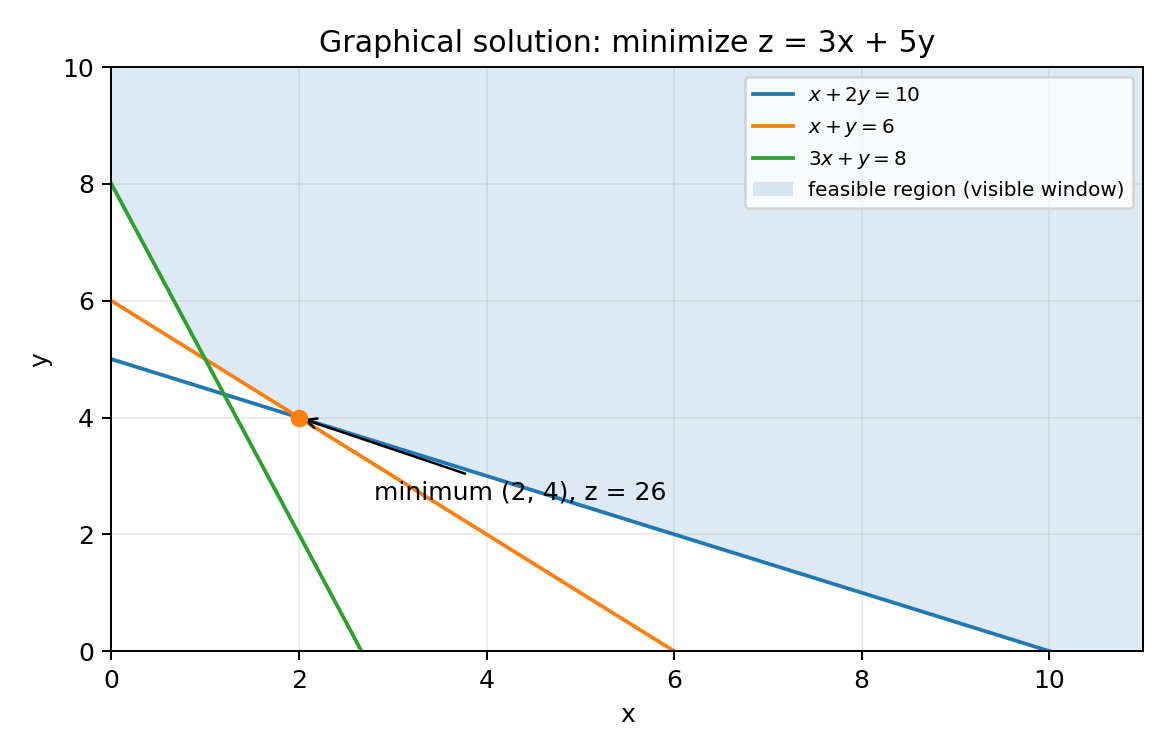
\includegraphics[width=0.92\linewidth]{12/figs/Q59.png}
    \end{figure}

    The following code verifies the solution.

    \begin{lstlisting}[frame=single, basicstyle=\rmfamily, escapeinside={(*@}{@*)}]
(*@\makebox[\dimexpr\linewidth-2\fboxsep-2\fboxrule\relax][c]{12/codes/Q59.py}@*)
    \end{lstlisting}



\item
\label{question:C12-Q58}
\label{question-short:C12-Q58} Evaluate:
\[
I=\int_0^{\pi/2}\frac{\cos^2 x}{1+3\sin^2 x}\,dx
\]

\par
\smallskip
\solution

Let
\[
f(x)=\frac{\cos^2 x}{1+3\sin^2 x}.
\]

Using the composite trapezoidal rule,

\begin{align*}
    T_n &= \frac{h}{2}\left[
    f(x_0)+2\sum_{i=1}^{n-1}f(x_i)+f(x_n)
    \right].
    \tag*{\eqref{formula:C12-Q58}}
\end{align*}

Taking $n=4$,

\[
h=\frac{\pi/2-0}{4}=\frac{\pi}{8}.
\]

The function values are

\[
\begin{array}{c|c}
x_i & f(x_i)\\ \hline
0 & 1.000000\\
\pi/8 & 0.593017\\
\pi/4 & 0.200000\\
3\pi/8 & 0.041129\\
\pi/2 & 0.000000
\end{array}
\]

Therefore,

\begin{align*}
    T_4 &= \frac{\pi}{8}\left[
    \frac12(1)+0.593017+0.200000
    +0.041129+\frac12(0)\right]\\
    &= 0.523918.
\end{align*}

    The following code verifies the solution.

    \begin{lstlisting}[frame=single, basicstyle=\rmfamily, escapeinside={(*@}{@*)}]
(*@\makebox[\dimexpr\linewidth-2\fboxsep-2\fboxrule\relax][c]{12/codes/Q61.py}@*)
    \end{lstlisting}


\item
\label{question:C12-Q59}
\label{question-short:C12-Q59} Evaluate:
\[
I=\int_0^{\pi/4}
\frac{\sin x+\cos x}{3+\sin 2x}\,dx
\]

\par
\smallskip
\solution

Let
\[
g(x)=\frac{\sin x+\cos x}{3+\sin 2x}.
\]

Using the composite trapezoidal rule,

\begin{align*}
    T_n &= \frac{h}{2}\left[
    g(x_0)+2\sum_{i=1}^{n-1}g(x_i)+g(x_n)
    \right].
    \tag*{\eqref{formula:C12-Q58}}
\end{align*}

Taking $n=4$,

\[
h=\frac{\pi/4-0}{4}=\frac{\pi}{16}.
\]

The function values are

\[
\begin{array}{c|c}
x_i & g(x_i)\\ \hline
0 & 0.333333\\
\pi/16 & 0.347616\\
\pi/8 & 0.352448\\
3\pi/16 & 0.353487\\
\pi/4 & 0.353553
\end{array}
\]

Therefore,

\begin{align*}
    T_4 &= \frac{\pi}{16}\bigg[
    \frac12(0.333333)+0.347616\\
    &\qquad+0.352448+0.353487
    +\frac12(0.353553)\bigg]\\
    &= 0.274299.
\end{align*}

    The following code verifies the solution.

    \begin{lstlisting}[frame=single, basicstyle=\rmfamily, escapeinside={(*@}{@*)}]
(*@\makebox[\dimexpr\linewidth-2\fboxsep-2\fboxrule\relax][c]{12/codes/Q62.py}@*)
    \end{lstlisting}

    \end{enumerate}


